\documentclass[11pt,letterpaper]{article}
\usepackage{style}

%% ------- INICIA DOCUMENTO ------
\begin{document}
\begin{titlepage}
\begin{center}
\begin{LARGE}
INSTITUTO POLITÉCNICO NACIONAL\\
\vspace*{0.15in}
ESCUELA SUPERIOR DE CÓMPUTO\\
\end{LARGE}
\vspace*{1.0in}
\begin{Large}
%% NOMBRE DE LA PRÁCTICA O EXAMEN
\textbf{TÉCNICAS DE CRUZA 1} \\  
\end{Large}
\vspace*{0.2in}
\begin{large}
\textit{Práctica 6}\\
\end{large}
\vspace*{1.0in}
\begin{large}
%% INTEGRANTES	
Dominguez de la Rosa Bryan\\
\vspace*{2.0in}
GRUPO 3CM5\\
\vspace*{0.2in}
Profesor: Morales Güitron Sandra Luz\\
\vspace*{1.5in}
\today
\vspace*{0.3in}
\end{large}
\rule{150mm}{0.1mm}\\

\end{center}
\end{titlepage}

%% --------- COMIENZA EL DESARROLLO DEL DOCUMENTO --------

\section*{Introducción}

En los sistemas biológicos, la cruza es un proceso complejo que ocurre entre parejas de cromosomas. Estos cromosomas se alinean, luego se fraccionan en ciertas
partes y posteriormente intercambian fragmentos entre sí.
En computación evolutiva se simula la cruza intercambiando segmentos de
cadenas lineales de longitud fija (los cromosomas).

\subsection*{Cruza por un Punto}
Esta técnica fue propuesta por Holland, y fue muy popular durante muchos
años. Hoy en día, sin embargo, no suele usarse mucho en la práctica debido a sus
inconvenientes. Puede demostrarse, por ejemplo, que hay varios esquemas que no
pueden formarse bajo esta técnica de cruza.

\begin{figure}[H]
	\centering
	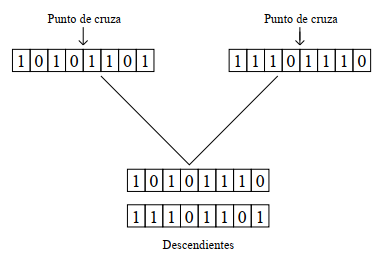
\includegraphics[scale = 0.7]{images/cup}
	\caption{Cruza por un punto.}
\end{figure}

\subsection*{Cruza por dos Puntos}
DeJong fue el primero en implementar una cruza de n puntos, como una
generalización de la cruza de un punto.
El valor n = 2 es el que minimiza los efectos disruptivos (o destructivos) de
la cruza y de ahí que sea usado con gran frecuencia.
No existe consenso en torno al uso de valores para n que sean mayores o
iguales a 3.
Los estudios empíricos al respecto proporcionan resultados que no
resultan concluyentes respecto a las ventajas o desventajas de usar dichos valores.
En general, sin embargo, es aceptado que la cruza de dos puntos es mejor que
la cruza de un punto.
Asimismo, el incrementar el valor de n se asocia con un mayor efecto disruptivo de la cruza.

\begin{figure}[H]
	\centering
	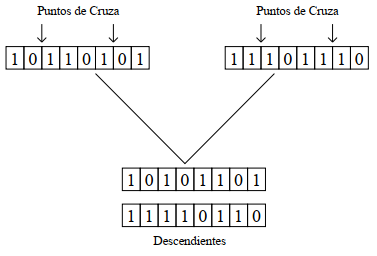
\includegraphics[scale = 0.7]{images/cdp}
	\caption{Cruza por dos puntos.}
\end{figure}

\subsection*{Cruza Uniforme}

Esta técnica fue propuesta originalmente por Ackley, aunque se le suele atribuir a Syswerda. En este caso, se trata de una cruza de n puntos, pero en la cual el número de puntos de cruza no se fija previamente.\\

La cruza uniforme tiene un mayor efecto disruptivo que cualquiera de las 2
cruzas anteriores. A fin de evitar un efecto excesivamente disruptivo, suele usarse
con P c = 0.5. Algunos investigadores, sin embargo, sugieren usar valores más pequeños de Pc.\\

Cuando se usa P c = 0.5, hay una alta probabilidad de que todo tipo de cadena
binaria de longitud L sea generada como máscara de copiado de bits.

\begin{figure}[H]
	\centering
	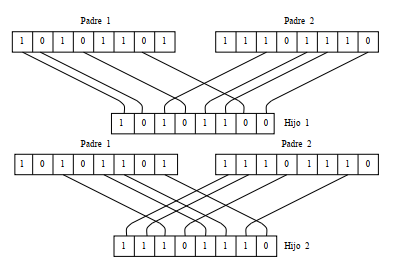
\includegraphics[scale = 0.7]{images/cu}
	\caption{Cruza uniforme.}
\end{figure}

\subsection*{Cruza Acentuada}

Esta técnica fue propuesta por Schaffer y Morishima, en un intento por
implementar un mecanismo de auto-adaptación para la generación de los patrones
favorables (o sea, los buenos bloques constructores) de la cruza.
En vez de calcular directamente la máscara (o patrón) de cruza, la idea es usar
una cadena binaria de “marcas” para indicar la localización de los puntos de cruza.
La idea fue sugerida por Holland, aunque en un sentido distinto.\\

La información extra que genera la cruza acentuada se agrega al cromosoma
de manera que el número y localizaciones de los puntos de cruza pueda ser objeto
de manipulación por el AG.
Por tanto, las cadenas tendrán una longitud del doble de su tamaño original.
La convención que suele adoptarse es la de marcar con ‘1’ las posiciones
donde hay cruza y con ‘0’ las posiciones donde no la hay.
Asimismo, se suelen usar signos de admiración para facilitar la escritura de
las cadenas.

\begin{figure}[H]
	\centering
	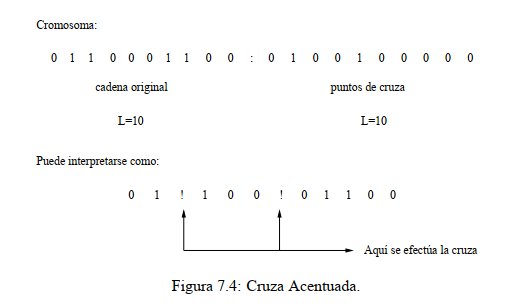
\includegraphics[scale = 0.7]{images/ca}
	\caption{Cruza acentuada.}
\end{figure}

\section*{Contenido}

Para la programación de los algoritmos de cruza se utilizó el lenguaje C++. A continuación se presentan las pruebas de cada algoritmo de cruza.

\subsection*{Cruza por un punto}

\begin{figure}[H]
	\centering
	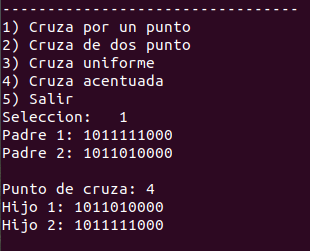
\includegraphics[scale = 1]{images/cruzaUnPunto}
	\caption{Cruza por un punto.}
\end{figure}

\subsection*{Cruza por dos puntos}

\begin{figure}[H]
	\centering
	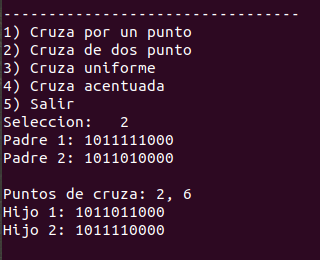
\includegraphics[scale = 1]{images/cruzaDosPuntos}
	\caption{Cruza por dos puntos.}
\end{figure}

\subsection*{Cruza uniforme}

\begin{figure}[H]
	\centering
	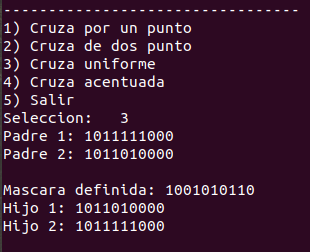
\includegraphics[scale = 1]{images/uniforme}
	\caption{Cruza uniforme.}
\end{figure}

\subsection*{Cruza acentuada}

\begin{figure}[H]
	\centering
	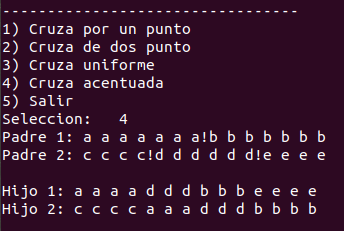
\includegraphics[scale = 1]{images/acentuada}
	\caption{Cruza acentuada.}
\end{figure}


\section*{Conclusión}

En los sistemas biológicos, la cruza es un proceso complejo que ocurre entre parejas de cromosomas. Estos cromosomas se alinean, luego se fraccionan en ciertas
partes y posteriormente intercambian fragmentos entre sí. El poder modelar ésto en un sistema computacional permite generar simulaciones de cómo se comportaría una población de individuos.


\end{document}


